\documentclass[12pt, a4paper]{article}

% Text languages
\usepackage[english, UKenglish, USenglish, american, british]{babel}

% Accents
%usepackage[latin1]{inputenc}

% Maths
\usepackage{mathtools}
\usepackage{amsmath,amsthm,amssymb}

% Double rows
%\usepackage{multirow}

% Math-mode symbol & verbatim
%\def\W#1#2{$#1{#2}$ &\tt\string#1\string{#2\string}}
%\def\X#1{$#1$ &\tt\string#1}
%\def\Y#1{$\big#1$ &\tt\string#1}
%\def\Z#1{\tt\string#1}

% A non-floating table environment.
%\makeatletter
%\renewenvironment{table}%
%   {\vskip\intextsep\parskip\z@
%    \vbox\bgroup\centering\def\@captype{table}}%
%   {\egroup\vskip\intextsep}
%\makeatother

%\DeclarePairedDelimiter\abs{\lvert}{\rvert}%
%\DeclarePairedDelimiter\norm{\lVert}{\rVert}%

% Swap the definition of \abs* and \norm*, so that \abs
% and \norm resizes the size of the brackets, and the 
% starred version does not.
%\makeatletter
%\let\oldabs\abs
%\def\abs{\@ifstar{\oldabs}{\oldabs*}}
%
%\let\oldnorm\norm
%\def\norm{\@ifstar{\oldnorm}{\oldnorm*}}
%\makeatother

% C++
\usepackage{listings}
\usepackage{xcolor}
\lstset { %
	language = C++,
	backgroundcolor=\color{black!5}, % set backgroundcolor
    basicstyle=\footnotesize,% basic font setting
    tabsize=4, % tab space width
    showstringspaces=false, % don't mark spaces in strings
    %numbers=left, % display line numbers on the left
    commentstyle=\color{green}, % comment color
    keywordstyle=\color{blue}, % keyword color
    stringstyle=\color{red} % string color
}

% https://www.overleaf.com/learn/latex/Page_size_and_margins
\usepackage{geometry}
\topmargin = -23pt
\oddsidemargin = 13pt
\headheight = 12pt
\headsep = 25pt
\textheight = 674pt
\textwidth = 426pt
\marginparsep = 10pt
\marginparwidth = 50pt
\footskip = 30pt
\marginparpush = 5pt
\hoffset = 0pt
\voffset = 0pt
\paperwidth = 597pt
\paperheight = 845pt

% Hyperlinks
\usepackage{hyperref}

% Figure
\usepackage{graphicx}
\usepackage{caption}
\usepackage{subcaption}
\usepackage{etoc}
% Example
\newtheorem{exmp}{Example}[section]
% Algorithms
%\usepackage[]{algorithm2e}
%\usepackage{algorithm}% http://ctan.org/pkg/algorithm
%\usepackage{algpseudocode}% http://ctan.org/pkg/algorithmicx
\usepackage{algpseudocode}

\renewcommand{\thefootnote}{\arabic{footnote}} % 1, 2, 3... (la que hay por defecto)

\setcounter{secnumdepth}{5}
\setcounter{tocdepth}{5}

%\titleformat{\paragraph}
%{\normalfont\normalsize\bfseries}{\theparagraph}{1em}{}
%\titlespacing*{\paragraph}
%{0pt}{3.25ex plus 1ex minus .2ex}{1.5ex plus .2ex}

\usepackage{float}
%--------------------------------------------------------------------------
\title{PARALLELISM}
\author{Roger Vilaseca Darné and Xavier Martín Ballesteros\\
  \small UNIVERSITAT POLITÈCNICA DE CATALUNYA\\
}
\date{10th December 2018}

\begin{document}
% Images
\graphicspath{ {./images} }

%\maketitle

\begin{titlepage}
	\centering
%	{\scshape\LARGE UNIVERSITAT POLITÈCNICA DE CATALUNYA \par}
	\vspace{1cm}
	{\scshape\Large UNIVERSITAT POLITECNICA DE CATALUNYA\par}
	\vspace{1.5cm}
	{\huge\bfseries PARALLELISM\par}
	\vspace{2cm}
	{\Large\itshape \textbf{Lab 4: Divide and Conquer parallelism with OpenMP: Sorting}\par}
	\vfill
	{\Large\itshape Roger Vilaseca Darne and Xavier Martin Ballesteros\break PAR4110\par}
	\vfill
	
\includegraphics[width=0.25\textwidth]{./images/UPC.png}\par\vspace{1cm}
	%supervised by\par
	%Dr.~Mark \textsc{Brown}

	\vfill

% Bottom of the page
	{\large 15th May 2019, Q2}
\end{titlepage}

%\abstract{Esto es una plantilla simple para un articulo en \LaTeX.}

%	*********************** ÍNDEX *********************
\setcounter{secnumdepth}{5}

\newpage
  \tableofcontents
\newpage

% Referència a una equació \ref{eq:area}).
% Referència a una secció \ref{sec:nada}
% Referència a una cita \cite{Cd94}.

\section{Introduction}

\section{Anlysis with \textit{Tareador}}

In order to study which is the best approach that we should use to parallelize the code (using the \textit{OpenMP} directives), a study about the task dependencies is needed.

In the following subsections, we will analyse the functions \textit{merge} and \textit{multisort} of the given code using \textit{Tareador} to see the potential parallelism they have and also their dependences. As both functions are recursive, it is very likely that we will be able to parallelise them.

The modified code can be found in the \textit{multisort-tareador.c} file, inside the codes directory.

\subsection{Merge Function}

The merge function is responsible for sorting two vectors, merging them into one. This is done using recursive calls that divide the vectors into smaller ones.

Our study in this function focuses on the two recursive calls done in the else fragment of the function. A task is created every time we make a recursive call to the function. As a consequence, some created tasks will also execute the basicmerge function.

To do that, we have used the \textit{tareador\_start\_task} and \textit{tareador\_end\_task} functions. The resulting code is shown below.

\begin{figure}[H]
\begin{lstlisting}
void merge(long n, T left[n], T right[n], T result[n*2], long start,
		   long length) {
    if (length < MIN_MERGE_SIZE*2L) {
        // Base case
        basicmerge(n, left, right, result, start, length);
    } else {
        // Recursive decomposition
        tareador_start_task("me1");
        merge(n, left, right, result, start, length/2);
        tareador_end_task("me1");

        tareador_start_task("me2");
        merge(n, left, right, result, start + length/2, length/2);
        tareador_end_task("me2");
    }
}
\end{lstlisting}

\label{code:merge_tareador}
\caption{Modified version of the merge function.}
\end{figure}


\subsection{Multisort Function}

The multisort function divides the input vector into four smaller vectors, apply a recursive call for each of them and them merges the 4 vectors into a big sorted one.

We will use the same strategy than in the merge function. This is, creating a task for each recursive call and for each call to the merge function.

We have also used the \textit{tareador\_start\_task} and \textit{tareador\_end\_task} functions. The code is the following:

\begin{figure}[H]
\begin{lstlisting}
void multisort(long n, T data[n], T tmp[n]) {
    if (n >= MIN_SORT_SIZE*4L) {
        // Recursive decomposition
        tareador_start_task("mu1");
        multisort(n/4L, &data[0], &tmp[0]);
        tareador_end_task("mu1");

        tareador_start_task("mu2");
        multisort(n/4L, &data[n/4L], &tmp[n/4L]);
        tareador_end_task("mu2");

        tareador_start_task("mu3");
        multisort(n/4L, &data[n/2L], &tmp[n/2L]);
        tareador_end_task("mu3");

        tareador_start_task("mu4");
        multisort(n/4L, &data[3L*n/4L], &tmp[3L*n/4L]);
        tareador_end_task("mu4");

        tareador_start_task("me1");
        merge(n/4L, &data[0], &data[n/4L], &tmp[0], 0, n/2L);
        tareador_end_task("me1");

        tareador_start_task("me2");
        merge(n/4L, &data[n/2L], &data[3L*n/4L], &tmp[n/2L], 0, n/2L);
        tareador_end_task("me2");


        tareador_start_task("me3");
        merge(n/2L, &tmp[0], &tmp[n/2L], &data[0], 0, n);
        tareador_end_task("me3");

    } else {
        // Base case
        basicsort(n, data);
    }
}
\end{lstlisting}

\label{code:multisort_tareador}
\caption{Modified version of the multisort function.}
\end{figure}

\subsection{Task dependency graph (TDG)}

We can clearly see that Figure \ref{fig:TDG} is divided into two parts: the multisort and the merge.

As we said before, in the multisort function we divide the input vector into 4 smaller vectors, until the vector size is smaller than $MIN\_SORT\_SIZE \times 4L$. This can be seen at the top of the figure, as we can see 4 different boxes (green, red, yellow and purple). Moreover, there is no data sharing between them, so we can execute them at the same time.

Then, there is a new recursion level inside each box. These four calls reach the limit value, so they do a \textit{basicmerge} call. Afterwards, we need the first two childs to terminate before executing the first merge call (and the same for the third and fourth childs with the second merge call). Thus, there exist a dependence between the recursive calls to multisort and the calls to the first two merge functions. Finally, the third merge call can be executed only when the previous two merge calls have terminated (another dependence).

On the other hand, in the merge function, we create tasks when the number of elements of the vector that we want to sort is bigger or equal than $MIN\_MERGE\_SIZE \times 2L$. We see in the figure that the two created tasks do not have any dependence between them. A \textit{basicmerge} call will be done when we reach the limit value.

\begin{figure}[H]
	\centering
	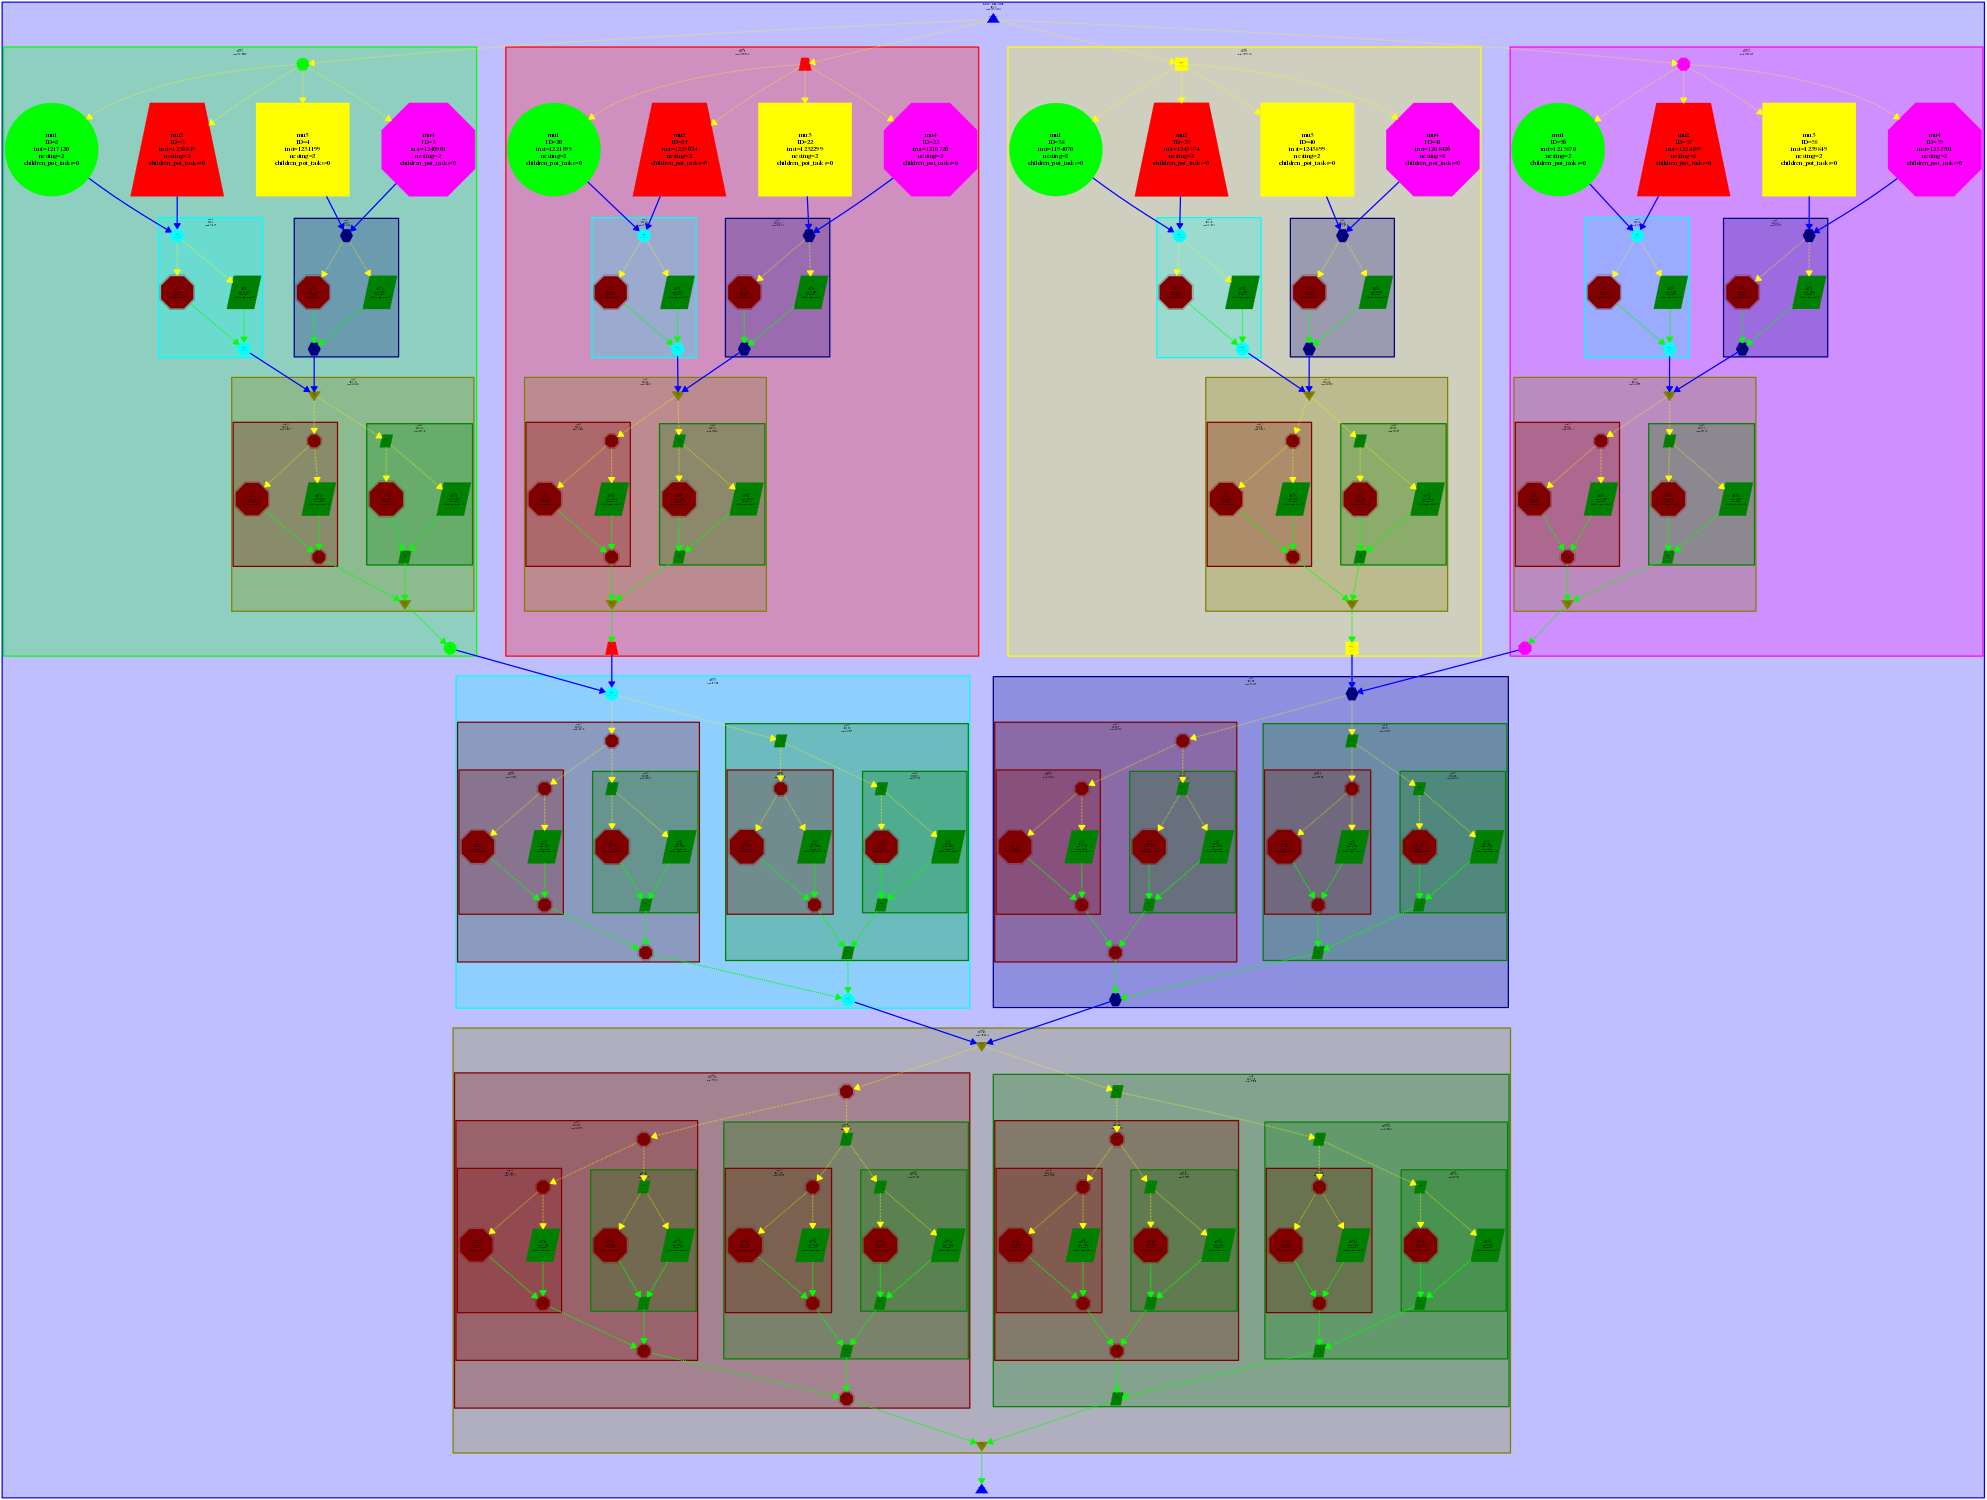
\includegraphics[scale=0.16]{./images/dependency_graph}
	
	\label{fig:TDG}
	\caption{Task dependency graph obtained using \textit{Tareador}.}
\end{figure}

With all these information, we can conclude that we can use a \textbf{Tree strategy} (generate a task for each recursive function) because there are no dependences between sibling tasks. Besides, we can also use a \textbf{Leaf strategy} (generate a task in each base case of the functions).

Furthermore, we must be careful about the synchronization we need between the multisort tasks and the merge ones because, as we said before, the first merge call depends on the first two multisort calls, the second merge call depends on the thids and fourth multisort calls and the third merge call depends on the previous two merge calls. Without synchronization we would have wrong results due to data racing.

\subsection{Parallel Performance and Scalability}

The following table shows the execution time and speed-up values obtained when varying the number of processors.

\begin{table}[H]
\centering
\begin{tabular}{ |c|c|c| } 
 \hline
 \textbf{Processors} & \textbf{Execution Time [ns]} & \textbf{Speed-Up} \\ 
 \hline
 \hline
	1	& 20334411001	& 1 \\
	 \hline
	2	& 10173716001	& 1.99872013323365 \\
	 \hline
	4	& 5086725001	& 3.99754478510288 \\
	 \hline
	8	& 2550595001	& 7.97241858979085 \\
	 \hline
	16	& 1289922001	& 15.7640624667507 \\
	 \hline
	32	& 1289909001	& 15.7642213406029 \\
	 \hline
	64	& 1289909001	& 15.7642213406029 \\
 \hline
\end{tabular}
 
 \label{tab:Scalability_S1}
\caption{Execution Time and Speed-Up varying the number of processors.}
\end{table}

We can see that until 16 processors, the results obtained are pretty close to the ideal ones. However, from 16 to infinite processors there is no improvement on the speed-up values. This is because in Figure \ref{fig:TDG} we see that the maximum number of tasks executed at the same time are 16. For this reason, using more than 16 processors will not have any impact on the execution time and speed-up.

\begin{figure}[H]
\hspace{-0.5cm}
\begin{subfigure}{.5\textwidth}
  \centering
  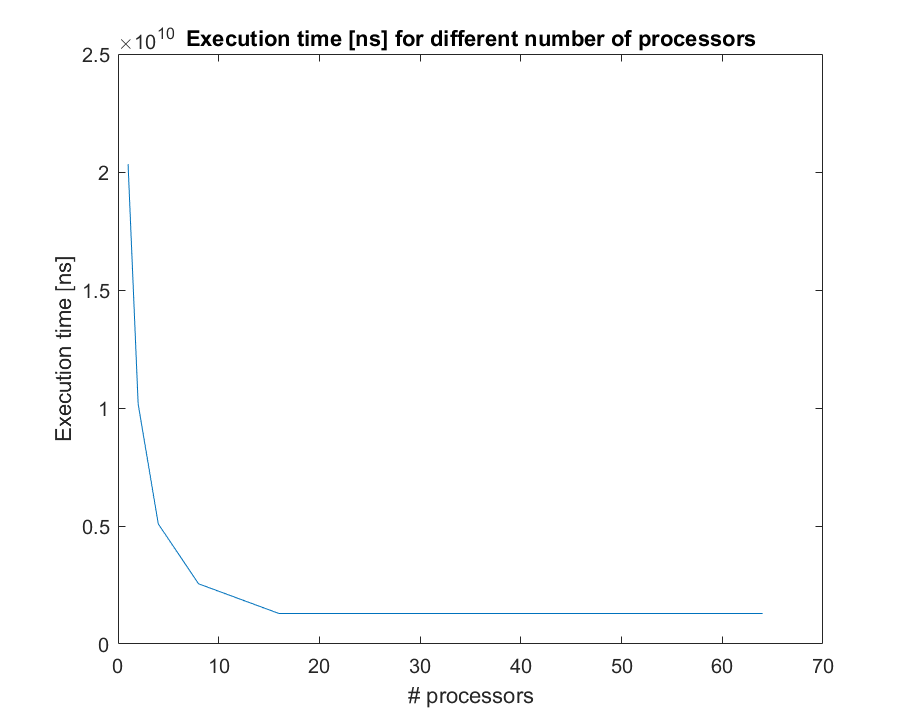
\includegraphics[width=1.10\linewidth]{./images/S1_plots/execution_time_line}
  
\end{subfigure}%
\begin{subfigure}{.5\textwidth}
  \centering
  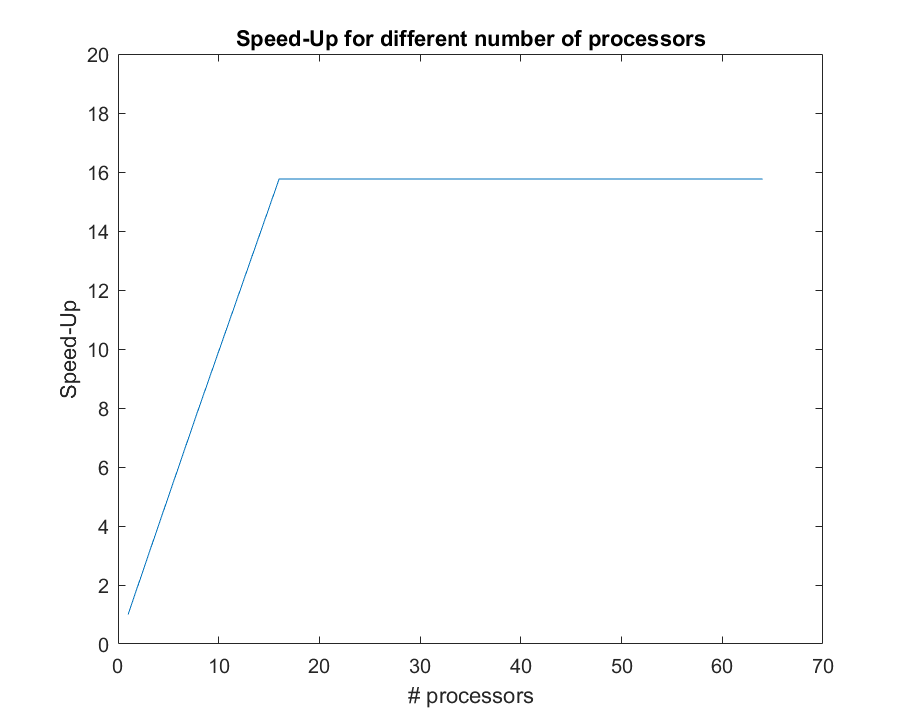
\includegraphics[width=1.10\linewidth]{./images/S1_plots/speedup_line}

\end{subfigure}
\caption{Execution Time and Speed-Up plots varying the number of processors.}
\end{figure}

\break

Include the relevant parts of the modified multisort-tareador.c code and comment where the
calls to the Tareador API have been placed. Comment also about the task graph generated and
the causes of the dependences that appear.

Write a table with the execution time and speed-up predicted by Tareador (for 1, 2, 4, 8, 16, 32
and 64 processors) for the task decomposition specified with Tareador. Are the results close to the
ideal case? Reason about your answer.


\section{Annex}

\subsection{Scalability anaysis: Traces using different number of processors}

\begin{figure}[H]
	\centering
	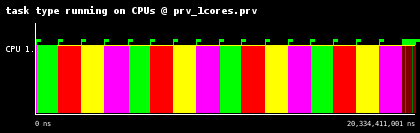
\includegraphics[scale=0.75]{./images/S1_scalability/S1_scalability_1}
	
	\label{fig_ann:S1_scalability_1}
	\caption{Execution flow of the code using 1 processor.}
\end{figure}





\begin{figure}[H]
	\centering
	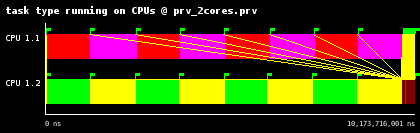
\includegraphics[scale=0.75]{./images/S1_scalability/S1_scalability_2}
	
	\label{fig_ann:S1_scalability_2}
	\caption{Execution flow of the code using 2 processors.}
\end{figure}





\begin{figure}[H]
	\centering
	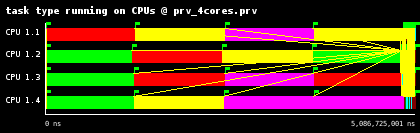
\includegraphics[scale=0.75]{./images/S1_scalability/S1_scalability_4}
	
	\label{fig_ann:S1_scalability_4}
	\caption{Execution flow of the code using 4 processors.}
\end{figure}





\begin{figure}[H]
	\centering
	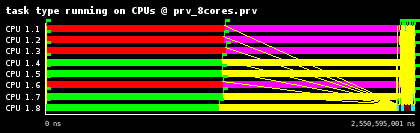
\includegraphics[scale=0.75]{./images/S1_scalability/S1_scalability_8}
	
	\label{fig_ann:S1_scalability_8}
	\caption{Execution flow of the code using 8 processors.}
\end{figure}





\begin{figure}[H]
	\centering
	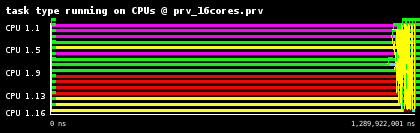
\includegraphics[scale=0.75]{./images/S1_scalability/S1_scalability_16}
	
	\label{fig_ann:S1_scalability_16}
	\caption{Execution flow of the code using 16 processors.}
\end{figure}





\begin{figure}[H]
	\centering
	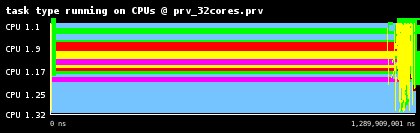
\includegraphics[scale=0.75]{./images/S1_scalability/S1_scalability_32}
	
	\label{fig_ann:S1_scalability_32}
	\caption{Execution flow of the code using 32 processors.}
\end{figure}





\begin{figure}[H]
	\centering
	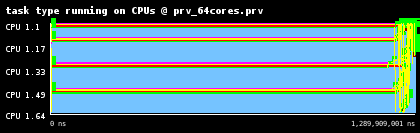
\includegraphics[scale=0.75]{./images/S1_scalability/S1_scalability_64}
	
	\label{fig_ann:S1_scalability_64}
	\caption{Execution flow of the code using 64 processors.}
\end{figure}

\end{document} 